\documentclass[12pt,a4paper]{article}
\usepackage[UTF8]{ctex}     %先引入ctex
\usepackage[utf8]{inputenc} %再引入inputenc
\usepackage{graphicx}
% \usepackage{lazylatex}
\usepackage{minted}
\usepackage{amsmath}
\usepackage{bookmark}
\usepackage{enumerate}
\usepackage{geometry}
\usepackage{tikz}
\usepackage{subfigure}
\usepackage{array}
\usepackage{colortbl}
% \tcbuselibrary{documentation}
\graphicspath{{img/}}
% 边距
\geometry{left=2.0cm,right=2.0cm,top=2.0cm,bottom=3.0cm}
% 大题
\newenvironment{problems}{\begin{list}{}{\renewcommand{\makelabel}[1]{\textbf{##1}.\hfil}}}{\end{list}}
% 小题
\newenvironment{steps}{\begin{list}{}{\renewcommand{\makelabel}[1]{(##1)\hfil}}}{\end{list}}
% 答
\providecommand{\ans}{\textbf{答}:~}
% 解
\providecommand{\sol}{\textbf{解}.~}

\setminted{breaklines,autogobble,frame=lines,framesep=2mm,fontsize=\scriptsize}

\begin{document}
\title{\normalsize \underline{计算机系统结构(A)}\\\LARGE 第 3 次作业}
\author{李子龙 518070910095}
\date{\today}
\maketitle

\begin{problems}
    \item[1] \textbf{直接映射}
     
\begin{tabular}{ccccccc}
Address Size & Cache size & Block Size &tag bits & Index bits & Offset bits & Bits per row \\
\hline
16& 4KB	    &4B	    &4	&10	&2	    &32+4+1\\
32& 32KB	&16B	& \bfseries 17& \bfseries	11& \bfseries	4&\bfseries	146\\
32& \bfseries 64KB	&\bfseries 16B	&16&	12&	\bfseries 4&\bfseries	145\\
64& 2048KB	&\bfseries 128B	&\bfseries 43&	14&	\bfseries 7&	1068\\
\hline
\end{tabular}

\item[2] \textbf{组相联映射}
\begin{enumerate}[(1)]
    \item 
    \begin{itemize}
        \item 地址长度:64MB=$2^{26}$(26位)
        \item 块内偏移长度:64B=$2^6$(6位)
        \item 行数:$\frac{\text{4KB}}{\text{64B}}=64=2^6$
        \item 组数:$\frac{64}{4}=16=2^4$(4位)
    \end{itemize}
   
    \begin{tikzpicture}
        \draw  (-6.5,1) rectangle (6.5,0);
        \draw  (3.5,1) rectangle (6.5,0);
        \draw  (1.5,1) rectangle (3.5,0);
        \node at (5,0.5) {块内偏移6位};
        \node at (2.5,0.5) {组编号4位};
        \node at (-2.5,0.5) {tag 16位};
    \end{tikzpicture}

    \item \begin{description}
        \item[写回策略] 修改位 1位;
        \item[LRU替换] 每组记录四块,需要LRU位 2位;
        \item[tag标记] 16位;
        \item[有效位]  1位;
        \item[数据]    64B; 
    \end{description}
    总计容量:
    \begin{equation*}
        64\times (16+1+1+2+64\times 8) = 34048\text{位}
    \end{equation*}
\end{enumerate}

    \item[3] \textbf{代码分析与高速缓存的性能}
    
    $\frac{128}{32}=4$行,共$\frac{4}{2}=2$组。

    \begin{tabular}{c|c|c|c|c|}
        \cline{2-5}
        & 标记 & 数据 & 标记 & 数据 \\
        \cline{2-5}
        0 & & & & \\
        \cline{2-5}
        1 & & & & \\
        \cline{2-5}
    \end{tabular}

    每块可以存储 4 个 \verb"long long" 数据。高速缓存访问的 32 次中,8次会miss,故高速缓存失效率为
    \begin{equation*}
        \frac{8}{32}\times 100 \% = 25\%
    \end{equation*}
    
    \item[4] \textbf{平均存储器访问时间(Average Memory Access Time:AMAT)}
     
    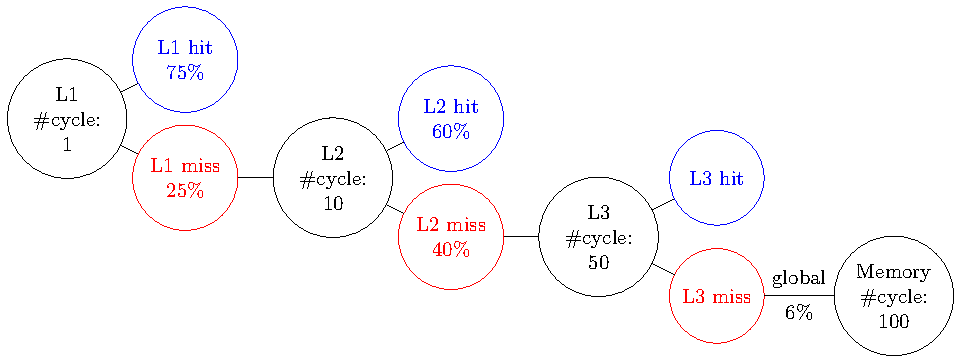
\includegraphics[width=\textwidth]{cache.pdf}

    \begin{align*}
        \mathit{AMAT}&=1+25\%\times (L2)\\
                    &=1+25\%\times (10+40\%\times (L3))\\
                    &=1+25\%\times(10+40\%\times(50+x\times 100))\\
                    &=1+25\%\times 10 + 25\%\times 40\% \times 50 + 25\%\times 40\% \times x\times 100\\
                    &=1+25\%\times 10 + 25\%\times 40\% \times 50 + 6\%\times 100\\
                    &=14.5
    \end{align*}

    \item[5] \textbf{虚拟存储器(Virtual Memory)}
    \begin{enumerate}[1)]
        \item TLB 将会对应更新该页对应的块,相当于将该页置入 TLB 中。
        \item 
        \begin{table}[h]
            \subfigure[Initial TLB]{
                \begin{tabular}{>{\ttfamily}c>{\ttfamily}cccc}
                    VPN	&PPN	&Valid	&Dirty&	LRU\\
                    0x01 & 0x11 & 1 & 1 & 0 \\
                    0x00 & 0x00 & 0 & 0 & 7 \\
                    0x10 & 0x13 & 1 & 1 & 1 \\
                    0x20 & 0x12 & 1 & 0 & 5 \\
                    0x00 & 0x00 & 0 & 0 & 7 \\
                    0x11 & 0x14 & 1 & 0 & 4 \\
                    0xac & 0x15 & 1 & 1 & 2 \\
                    0xff & 0x16 & 1 & 0 & 3 
                \end{tabular}
            }
            \subfigure[Read \texttt{0x11f0}]{
                \begin{tabular}{>{\ttfamily}c>{\ttfamily}cccc}
                    VPN	&PPN	&Valid	&Dirty&	LRU\\
                    0x01 & 0x11 & 1 & 1 & 1 \\
                    0x00 & 0x00 & 0 & 0 & 7 \\
                    0x10 & 0x13 & 1 & 1 & 2 \\
                    0x20 & 0x12 & 1 & 0 & 5 \\
                    0x00 & 0x00 & 0 & 0 & 7 \\
                    \rowcolor{gray!50} 0x11 & 0x14 & 1 & 0 & 0 \\
                    0xac & 0x15 & 1 & 1 & 3 \\
                    0xff & 0x16 & 1 & 0 & 4 
                \end{tabular}
            }
            \subfigure[Write \texttt{0x1301}]{
                \begin{tabular}{>{\ttfamily}c>{\ttfamily}cccc}
                    VPN	&PPN	&Valid	&Dirty&	LRU\\
                    0x01 & 0x11 & 1 & 1 & 2 \\
                    \rowcolor{gray} 0x13 & 0x17 & 1 & 1 & 0 \\
                    0x10 & 0x13 & 1 & 1 & 3 \\
                    0x20 & 0x12 & 1 & 0 & 6 \\
                    0x00 & 0x00 & 0 & 0 & 7 \\
                    0x11 & 0x14 & 1 & 0 & 1 \\
                    0xac & 0x15 & 1 & 1 & 4 \\
                    0xff & 0x16 & 1 & 0 & 5 
                \end{tabular}
            }
            \subfigure[Write \texttt{0x20ae}]{
                \begin{tabular}{>{\ttfamily}c>{\ttfamily}cccc}
                    VPN	&PPN	&Valid	&Dirty&	LRU\\
                    0x01 & 0x11 & 1 & 1 & 3 \\
                    0x13 & 0x17 & 1 & 1 & 1 \\
                    0x10 & 0x13 & 1 & 1 & 4 \\
                    \rowcolor{gray!50} 0x20 & 0x12 & 1 & 1 & 0 \\
                    0x00 & 0x00 & 0 & 0 & 7 \\
                    0x11 & 0x14 & 1 & 0 & 2 \\
                    0xac & 0x15 & 1 & 1 & 5 \\
                    0xff & 0x16 & 1 & 0 & 6 
                \end{tabular}
            }
            \subfigure[Write \texttt{0x2332}]{
                \begin{tabular}{>{\ttfamily}c>{\ttfamily}cccc}
                    VPN	&PPN	&Valid	&Dirty&	LRU\\
                    0x01 & 0x11 & 1 & 1 & 4 \\
                    0x13 & 0x17 & 1 & 1 & 2 \\
                    0x10 & 0x13 & 1 & 1 & 5 \\
                    0x20 & 0x12 & 1 & 1 & 1 \\
                    \rowcolor{gray} 0x23 & 0x18 & 1 & 1 & 0 \\
                    0x11 & 0x14 & 1 & 0 & 3 \\
                    0xac & 0x15 & 1 & 1 & 6 \\
                    0xff & 0x16 & 1 & 0 & 7 
                \end{tabular}
            }
            \subfigure[Read \texttt{0x20ff}]{
                \begin{tabular}{>{\ttfamily}c>{\ttfamily}cccc}
                    VPN	&PPN	&Valid	&Dirty&	LRU\\
                    0x01 & 0x11 & 1 & 1 & 4 \\
                    0x13 & 0x17 & 1 & 1 & 2 \\
                    0x10 & 0x13 & 1 & 1 & 5 \\
                    \rowcolor{gray!50} 0x20 & 0x12 & 1 & 1 & 0 \\
                    0x23 & 0x18 & 1 & 1 & 1 \\
                    0x11 & 0x14 & 1 & 0 & 3 \\
                    0xac & 0x15 & 1 & 1 & 6 \\
                    0xff & 0x16 & 1 & 0 & 7 
                \end{tabular}
            }
            \subfigure[Write \texttt{0x3415} at final state]{
                \begin{tabular}{>{\ttfamily}c>{\ttfamily}cccc}
                    VPN	&PPN	&Valid	&Dirty&	LRU\\
                    0x01 & 0x11 & 1 & 1 & 5 \\
                    0x13 & 0x17 & 1 & 1 & 3 \\
                    0x10 & 0x13 & 1 & 1 & 6 \\
0x20 & 0x12 & 1 & 1 & 1 \\
                    0x23 & 0x18 & 1 & 1 & 2 \\
                    0x11 & 0x14 & 1 & 0 & 4 \\
                    0xac & 0x15 & 1 & 1 & 7 \\
                    \rowcolor{gray} 0x34 & 0x19 & 1 & 1 & 0 
                \end{tabular}
            }
        \end{table}
    \end{enumerate}  
\end{problems}

\end{document}